\subsection{Visão Geral}
Este teste visou verificar a aplicabilidade do sensor laser Faro Focus 3D X330
no ambiente de trabalho da turbina. O dipositivo apresenta sensibilidade a
ambientes onde haja alta umidade, pois opera com um sistema de lentes e lasers
e, caso apresente condensação em um desses componentes, o resultado final de
sensoriamento pode ser prejudicado. Por esse motivo foi necessário realizar
testes com o sistema para analisar a viabilidade técnica de se usar o sensor
para a aplicação do projeto EMMA. 


\subsection{Equipamentos utilizados}

\begin{enumerate}
\item Faro Focus 3D X330 
\item Tripé de apoio
\item Esferas Reflexivas com base magnética
\end{enumerate}

\begin{figure}[h!]
\centering
	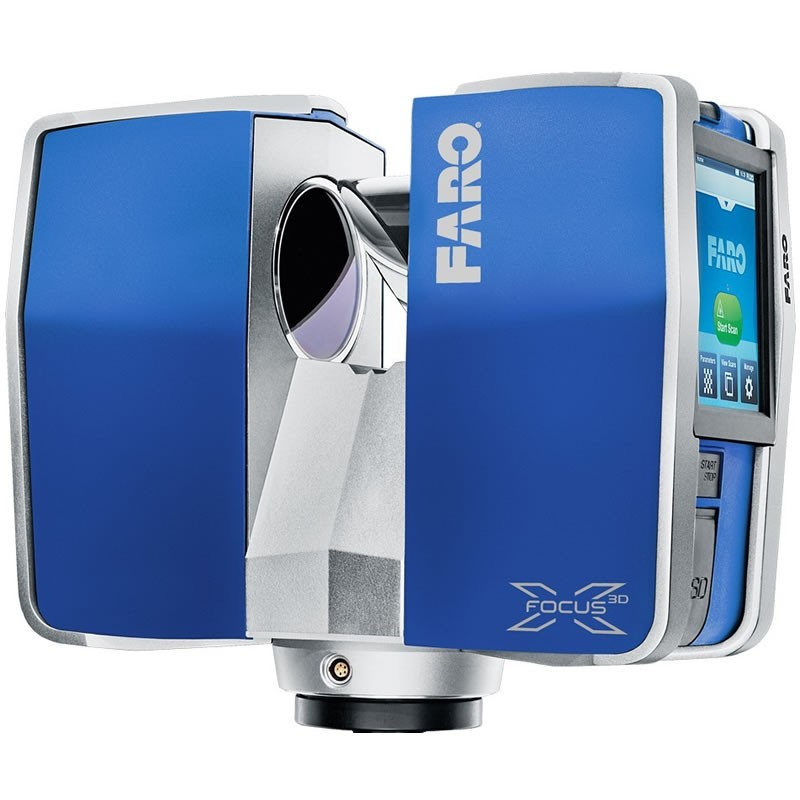
\includegraphics[width=0.4\columnwidth]{figs/faro/sensor}
	\caption{Sensor Faro Focus 3D X330.}
	\label{fig::sensor}
\end{figure}

\begin{figure}[h!]
\centering
	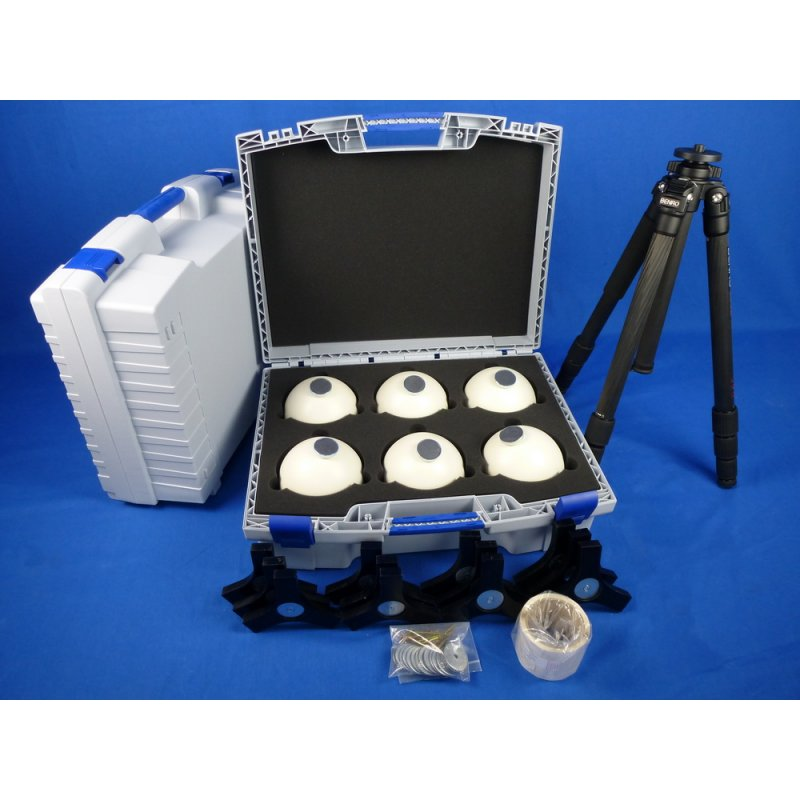
\includegraphics[width=0.5\columnwidth]{figs/faro/kit}
	\caption{Conjunto de esferas Reflexivas e tripé}
	\label{fig::kit}
\end{figure}


\subsection{Dados dos equipamentos}

\begin{itemize}
  \item Faro Focus 3D X300
  \begin{itemize}
    \item \textbf{Alcance:} 0,6 m - 330 m
    \item \textbf{Velocidade de medição (pts/seg.):}s 122.000 / 244.000 /
    488.000 / 976.000
    \item \textbf{Erro de alcance:} $\pm 2 mm$
    \item \textbf{Campo de visão vertical (vertical/horizontal):} 300$^o$ /
    360$^o$
    \item \textbf{Tamanho do passo (vertical/horizontal):} 0,009$^o$
    \item \textbf{GPS:} Receptor GPS integrados
    \item \textbf{Peso:} 5,2 kg
    \item \textbf{Temperatura ambiente:} $5^o - 40^o C$
    \item \textbf{Umidade:} Sem condensação
  \end{itemize}
\end{itemize}

\subsection{Procedimento}

Quatro esferas reflexivas foram distribuidas pelo ambiente, ficando três na
succção, próximas ao aro câmara, e uma sobre o distribuidor. Em seguida, foram
coletados dados a partir de 4 pontos com o sensor montado sobre o tripé. Três
dos pontos de coleta foram na sucção, aproximadamente igualmente espaçados e
alinhados com o eixo da turbina, e um entre a turbina e o distribuidor.

\subsection{Resultados}

A visualização dos dados coletados pelo scanner confirmou que não houve
condensação nos espelhos, apesar da alta humidade do local. Uma pequena
apresetanção em vídeo (figura \ref{fig::video}) dos dados coletados e uma
reconstrução em CAD da pá (figura \ref{fig::pa}) da turbina também foram
alcançadas.

\begin{figure}[h!]
\centering
	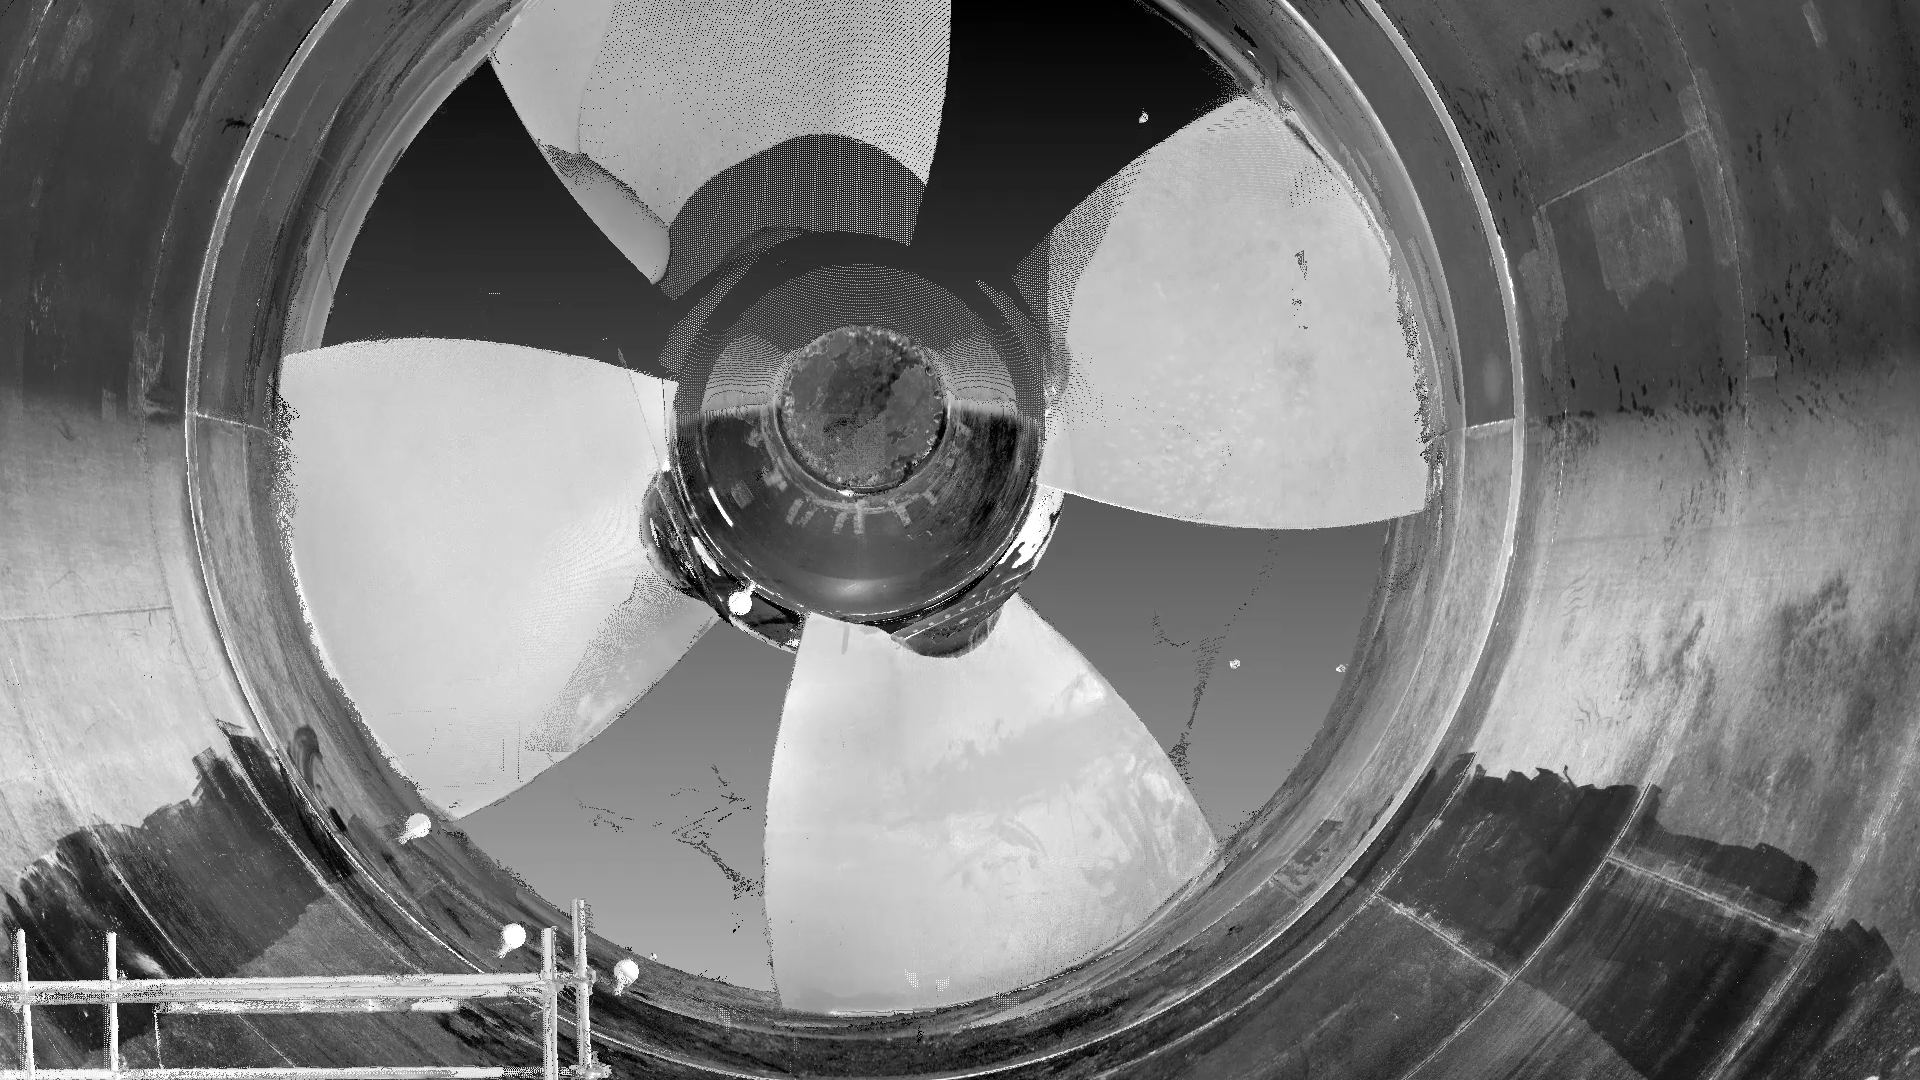
\includegraphics[width=0.4\columnwidth]{figs/faro/recorte_video}
	\caption{Recorte do vídeo dos dados adquiridos durante o teste.}
	\label{fig::video}
\end{figure}

\begin{figure}[h!]
\centering
	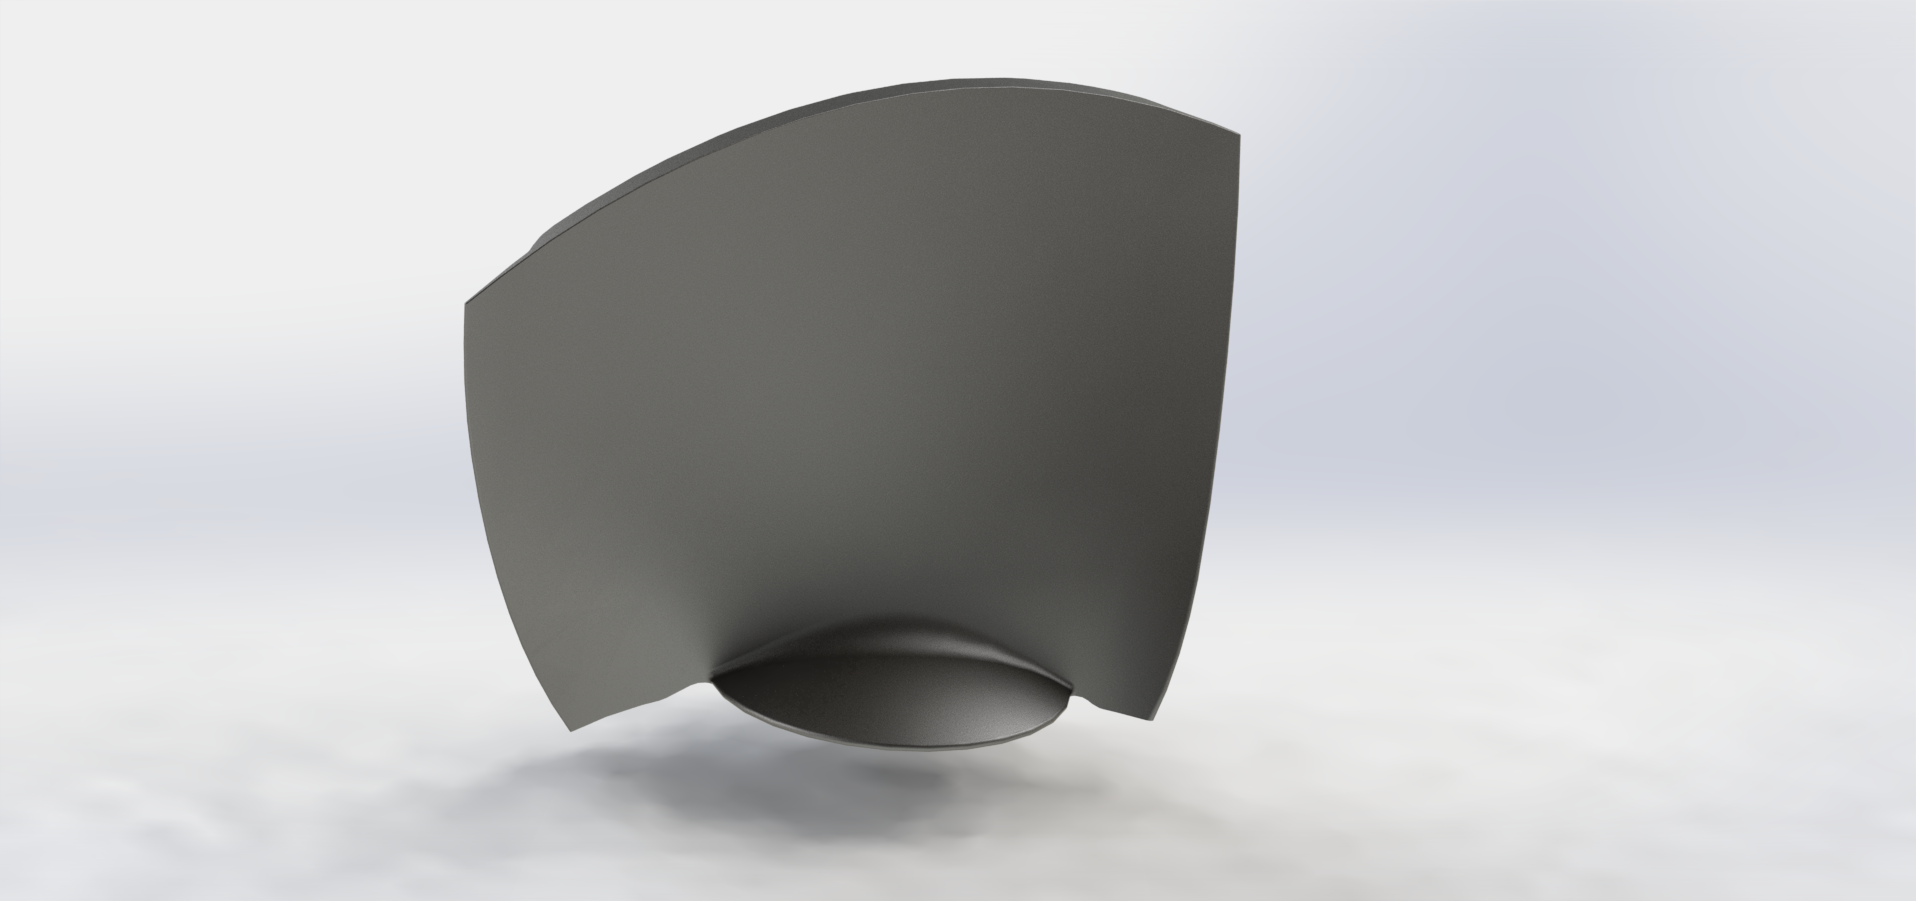
\includegraphics[width=0.5\columnwidth]{figs/faro/Pa_Real_Render_04}
	\caption{Reconstrução em CAD da pá com os dados do teste.}
	\label{fig::pa}
\end{figure}



\subsection{Conclusões}

De acordo com os resultados obtidos através desse teste, a hipótese de uso do
Faro Focus 3D X300 no ambiente da turbina foi confimada.
